\chapter{Non-obtrusive detection of emotions}
\label{ch:discussion}

The initial chapters of this thesis presented the theoretical foundations and the work needed to create a novel method for remote detection of emotions of users during the interaction with games. As highlighted by previous research, the understanding of human emotions, as well as the process of automatically detecting them, is the aim of several researchers in a many different fields. As detailed in Chapter \ref{ch:literature-games}, different theories have been proposed to model and study emotions in a variety of contexts, including those related to games. A considerable share of those theories is based on the human physiology, connecting emotional reactions to psychophysiological signals, e.g. HR and facial activity. Several approaches have been proposed to put such models and theories into practice to achieve the ultimate goal of detecting what a person is feeling. Chapters \ref{ch:literature-face} and \ref{ch:literature-physiological}, for instance, describe the connection between emotions and their manifestations in the body, particularly the process of mapping measurable psychophysiological signals into an emotional state.

Emotion detection is a complex and multidisciplinary problem that demands knowledge from many different areas. In this thesis, focus has been given to the field of games research. Results and contributions of this research are aimed at and discussed under the light of games research, however they are likely to be useful for scholars in other fields as well. This chapter presents and discusses the outcomes of this research, which is focused on creating a non-obtrusive method for emotion detection, particularly in the context of games. The following sections also present insights obtained during the systematic investigation and development of the proposed method, including a discussion on how they relate to games research and other areas.

\section{Game-based model for emotion detection}

Commonly the process of detecting emotions using psychophysiological signals relies on mapping the patterns of such signals into an emotional state. As pointed by the literature review conducted in this thesis, a validated way of doing it is by measuring the changes of psychophysiological signals caused by the interaction between user and emotion elicitation materials. Generally the process involves three main parts: emotion elicitation, signal acquisition and the mapping of such signals into an emotional state. Simply put, subjects are exposed to materials that are likely to produce certain emotional reactions, e.g. video and images depicting sad events, followed by observations of how the signals of interest, e.g. HR, change in accordance. Finally the emotion detection is performed by a technique aimed at producing a model to map the changes of those signals into emotional states, e.g. machine learning model like neural networks. The literature review presented in this thesis shows a myriad of different approaches used in each of the previously mentioned parts.

The majority of previous work focuses on producing a group model, where data from several individuals is used to created a trained machine able to detect emotions of any other subject outside the training population. Contrary to the established notion that a group model is better, this research investigated the venue of a user-tailored approach. As pointed by previous findings \parencite{something}, a model trained on data of a given person might be better at predicting the emotional state of such person. This is motivated by the fact that people are different in many aspects, including cultural and personal expectations \parencite{some}. Furthermore it is reasonable to believe that those individual characteristics might be preserved and better accounted for in a method that uses a user-tailored model as opposed to a group model to detect emotions. In this thesis, both the emotion elicitation process and the mapping of psychophysiological signals into emotional states were focused on the notion of the individual as opposed to the group.

\subsection{Calibration games as emotion elicitation}

%When games are used, they are usually gamified version of cognitive tests, or games featuring a well defined difficulty curve, e.g. easy/hard levels. Users have different gaming skills and expectations, so a game designed to be elicitate stresss might not be perceived as such by some users.

%, while previous work explored the use of games as elicitation sources for recognizing user emotions, relying on the emotional states a person can experience \citep{mandryk2006continuous} and which physiological signals are better predictors of such states \citep{jerritta2011physiological},

Previous works have used several different emotion elicitation materials, mainly images and videos, and less often game-related elements. Those material, however, lack a more user-tailored approach for studying the variations of signals. When games are used, emotional states such as stress and boredom are often inducted by administering a game with the same particular setup, e.g. high/low difficulty, to all subjects. People respond differently to media according to their personality \parencite{ravaja2004effects}, and they differ in social, learning and play styles \parencite{goldberg1993structure}. A game session labeled as stressful, for instance, assumes that all subjects have the same expectations and behave similarly, which dilutes the individuality of each person as some might experience the interaction as not being stressful as intended. Additionally the analysis usually involves the interaction of subjects with some game levels (from the same game) featuring a constant difficulty scale, which does not contemplate the variations of signals in a context where the game difficulty is constantly increasing in the same game level/session.

Investigation of better game-based emotion elicitation materials was one of the main aspects of this research. Aiming to properly elicitate particular emotional states on each user, this research introduced the novel idea of calibration games. As detailed in Section \ref{sec:experiment1-games-elicitation} (on page \pageref{sec:experiment1-games-elicitation}), calibration games are carefully designed and developed games that have a difficulty level that constantly and linearly progresses over time without a pre-defined stopping point. At the beginning the games are highly predictive, without novelties, changes or surprises and with emphasis on the passage of time during a wait, which leads to an emotional state of boredom \parencite{van2010behave,koster2013theory,schell2014art}. The game difficulty is then periodically increased until the subject is not able to cope with the challenges at hand, which happens at different times for different users. The ever-growing game difficulty leads to an emotional state of stress towards the end of the interaction, accounting for the different expectations and gaming skill of a wide range of users.

Sections \ref{sec:experiment1-study1} and \ref{sec:experiment1-study2} presented a detailed analysis regarding how responses related to physiological activity, i.e. HR and facial actions (FA), relate to emotional states in a game context featuring constant changes in difficulty (calibration games). Results show that a calibration games is a valid emotion elicitation material which accounts for personal differences among subjects when inducing emotional states of stress and boredom. Using the proposed calibration games, it was possible to observe and confirm with statistical significance variations of HR and naked-eye recognizable FA that happened during the interactions with the games, especially under situations that were designed to provoke boredom and stress. Those findings were an essential part of the user-tailored method proposed in this thesis, since they proved that calibration games can be used as emotion elicitation material. Another important factor is the nature of the calibration games when compared to other emotional stimuli, e.g. images or videos. The use of images, videos or text as content to produce the emotional stimuli is less likely to produce the reactions of a real gaming session. In a game, users are in charge of actions, which are bound to have consequences. A bad judgment might cause the main character to get hurt, or a right movement might produce a reward. This feedback loop is happening constantly in a game, likely producing emotional reactions on the user. It is plausible to believe that the calibration games present a more sophisticated interaction through their game mechanics, as opposed to the simplistic, or even inexistent, interaction between users and images/videos, for instance. Consequentially the use of calibration games is likely to create a deeper emotional connection between users and the emotion elicitation material, resulting in clear and observable changes in psychophysiological signals.

\subsection{Remote readings of psychophysiological signals}

Several of the works found in the literature rely on physical sensors to acquire the signals used in the emotion detection model. Physical sensors are not ideal since they require a cumbersome setup and might disturb the user experience, i.e. invalidate the use of a finger or hand. Use of remote sensing to acquire psychophysiological signals, a non-obtrusive approach of data collection, is mentioned as a promising solution for that problem. A complete non-obtrusive method for signal acquisition, however, is a complex and challenging problem, particularly in a context involving games.

One of the signals that are commonly acquired using remote and non-obtrusive approaches is facial activity. Chapter \ref{ch:literature-face} (on page \pageref{ch:literature-face}) describes in details techniques for facial analysis and the approaches using them for emotion detection. As mentioned in the chapter, results indicate that facial analysis is a promising source of information to be used in the process of emotion detection. Additionally  the combined use of facial and body features (multimodal emotion recognition) is known to perform better than using either one alone \parencite{zacharatos2014automatic}. Following the findings of previous work, the present thesis used facial activity as an important signal in the emotion detection process. A novel method for automated analysis of facial cues from videos was developed, as explained in Section \ref{s:experiment1-study4} (on page \pageref{s:experiment1-study4}). Empirical results of such method show its potential for detecting stress and boredom of players in games. The method is based on Euclidean distances between automatically detected facial points, designed to be robust enough to correctly perform facial analysis even when users are naturaly interacting with games. In such case, players behave naturally as they play, e.g. moving, laughing and speaking. Evaluations of the method were performed experimentally using game-based emotion elicitation, which properly contextualized the efficiency of the method in the field of games research. Results presented in Section \ref{s:experiment1-study4} confirm the method has the potential to differentiate emotional states of boredom and stress of players, however the natural behavior of users during the interaction with the games is a significant factor impacting the analysis.

%. Secondly we present the results of an automated facial analysis performed on subjects of our experiment, who interacted with different games under boring and stressful gameplay conditions. Our results show that values of facial features detected during boring periods of gameplay are different from values of the same facial features detected during stressful periods of gameplay. Even though the nature of our games, i.e. 2D and casual, and the sample size (N=20) could be limiting factors for the generality of the evaluation of our method, we believe our population of experimental subjects is diverse and our results are still promising. Our study contributes with results that can guide further investigation regarding emotions and facial analysis in gaming contexts. .

Another signal acquired using remote and non-obtrusive approaches is HR and its derivatives. Chapter \ref{ch:literature-rppg} (on page \pageref{ch:literature-rppg}) details the progress that has been made in the remote estimation of physiological signals, particularly the use of rPPG to estimate HR. Despite the potential rPPG has to eliminate physical sensors completely, its use is considerably impacted by the natural behavior of users. As presented in Section \ref{s:experiment1-study3} (one page \pageref{s:experiment1-study3}), rPPG estimations of HR are sensitive to noise caused by movement, facial expressions or changes in illumination (e.g. screen activity reflected on user's face), which are all likely to happen in gaming sessions. Those interferences might produce unreliable measurements of the HR signal, resulting in misleading data. Despite those limitations, the use of remote measurement of physiological signals, such as rPPG, has already been applied to emotion detection. Signals as HR and HRV were used to remotely detect stress \parencite{mcduffcogcam, mcduff2014improvements, bousefsaf2013remote}, for instance. In the majority of the cases, subjects are typically instructed to stay still \parencite{rouast2016remote}, which improves the accuracy of the rPPG technique. In some other cases, however, authors evaluate the accuracy of the HR estimation under scenarios where subjects are instructed to act naturally. Despite the fact that such works present experiments where subjects are told to behave naturally, their accuracy evaluation is based on artificial or simple human-computer interactions. Subjects are idly staring at the camera \parencite{zhao2013remote,hsu2014learning}, faking an interaction with a computer \parencite{poh2010non}, working on a task, i.e. make a website \parencite{monkaresi2014machine} or mentally subtract numbers \parencite{mcduff2014remote}, or performing arbitrary movements \parencite{tran2015robust}, e.g. head rotation in different degrees. Following the results of previous work, rPPG estimations were used in this thesis as a method for remote acquisition of a HR signal. Extensive evaluations were conducted to establish the reliability of remote HR measurements under situations with natural behavior, where users were not instructed to behave differently than what they usually do. Analysis of the accuracy of remote HR estimations clearly established the limitations of the rPPG technique, showing how it is affected when used to estimate HR of users interacting with games. 

%are presented and discussed. The main contribution of this paper is the accuracy evaluation of an established rPPG technique within the context of gaming sessions where users behave naturally instead of following movement constraint rules, e.g. remain still. Our results provide researchers with information related to the reliability of a remote HR measurement technique when applied to contexts where users behave more naturally

%is drastically impacted by noise introduced by the movement of users. Previous research countered this problem by instructing users to stand still during any interaction, or by limiting the complexity of such interactions, e.g. using images/videos as emotion elicitation materials, not games. In the present research, effort has been put to apply rPPG in a context involving users behaving naturally while interacting with games. Results

\section{Multifactorial emotion detection}

Something.


\section{Insights outside games research}

Here I will present some of the insights I gained during the whole process. I can mention how HR actually changes in the calibration games, hinting that researchers could use this information to create better models, for instance. I will also mention how the use of remote estimations of HR is a good tool, however it is extremely affected by natural movement (as detailed in study 3).

\section{Enhancing questionnaires in game research}

Here I will connect my research with its practical use. I will try to show how it can be used as a tool to enhance the use of questionnaires in game research. I could say that this approach can be used to replace questionnaires, but our numbers do not allow such a bold statement at the moment.


%\begin{figure}[h]
%    \centering
%    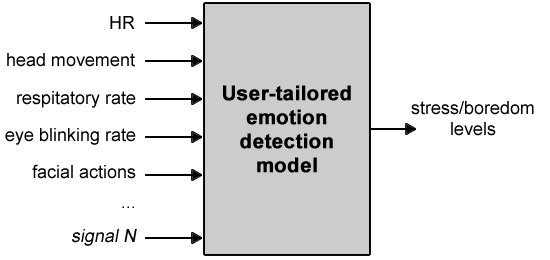
\includegraphics[width=0.6\textwidth]{figures/model-inputs-set.png}
%    \caption{Overall structure of the user-tailored emotion detection model regarding input (user signals) and output (stress/boredom levels).}
%    \label{fig:model-inputs-set}
%\end{figure}

%The user-tailored model proposed for this research might have $N$ input signals, varying from physiological ones, e.g. HR, to non-physiological ones, e.g. facial actions and head movements. Figure \ref{fig:model-inputs-set} illustrates the overall structure of the model. In order to be used in the model, an input signal needs to be supported by previous work regarding emotion detection, as well as be validated within the process of the proposed game-based calibration phase. Time and scope constraints limit the amount of input signals that can be implemented, evaluated and used in this research. As a consequence, a study will be conducted to investigate, validate and initially implement two of those signals into the proposed model: HR and facial activity (which includes head movement, lips activity, etc).

%The techniques and works presented in chapter \ref{ch:literature-face}, which relate to face detection and emotion estimation, suggest that facial analysis is an important component of a multifactorial emotion detection model. Empirical analysis of the data from the first experiment also suggest that individualities regarding facial activities do exist and could be used to estimate emotional states on a user-tailored basis \parencite{bevilacqua2016variations}. As described in section \ref{ch:literature-face-emotion-detection}, facial actions, head movement, lips/eye/mouth activity and distance measurements of detected facial landmarks are viable and proven sources of information for emotion detection.

%Regarding physiological signals, results indicate that the average HR mean for players during the last minute of gameplay is greater than the average HR mean during the second minute of gameplay (chapter \ref{ch:experiment1}, section \ref{s:experiment1-study3}). The findings are aligned with and reinforce previous research that indicates higher HR mean during stressful situations in a gaming context. The findings also suggest that changes in the HR during gaming sessions is a promising indicator of stress.

%The study will involve the definition of how those two signals will be used as inputs for the model. Facial actions, for instance, will probably be detected and measured by the euclidian distance of the facial landmarks. A vector containing the distances will be evaluated as the input for the model. Regarding the HR, its mean and standard deviation during a particular analysis window will be evaluated as input for the model. A software for the detection of those two signals will be created and used to analyse the video recordings of the first experiment (chapter \ref{ch:experiment1}). The inclusion or exclusion of a component of a signal, e.g. variations of the distances of the lips landmark points, will be based on the accuracy to detect them and the frequency they appear in boring and stressful part of the calibration games.
